%--------------------------------------------------
\section{Modelo de entidades del negocio}

\begin{figure}[htbp!]
		\centering
			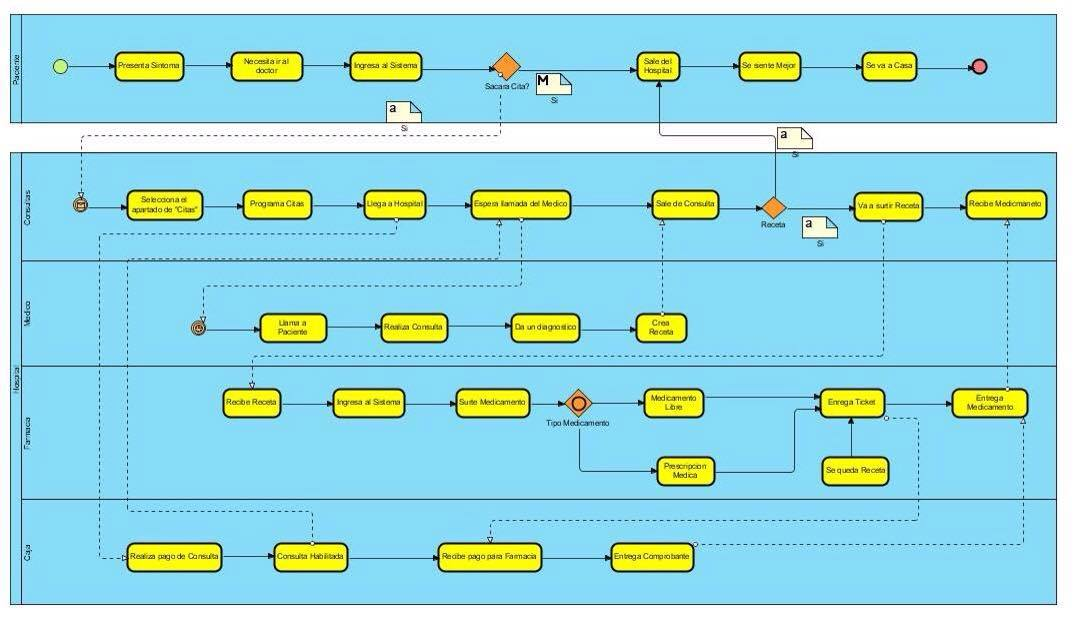
\includegraphics[scale=0.4]{images/bpm}
		\caption{Modelo BPMN}
\end{figure}


%--------------------------------------------------
\section{Descripci�n de atributos}

Describa para cada Entidad sus atributos y su significado. Por ejemplo:

% - - - - - - - - - - - - - - - - - - - - - - - - -
\subsection{Atributos de ''Paciente''}

\begin{description}
	\item[No. registro: ] Es ua cadena de caracteres el cual sirve para identificar al cliente y sea mas facil su busqueda en el sistema.
	\item[Nombre: ] Nombre del paciente.
	\item[Status: ] Corresponde al estado del alumno. Debe ser uno de los valores permitidos para ``Status del Alumno'' (ver glosario).
\end{description}

\subsection{Atributos de ''Doctor''}
\begin{description}
    \item[Matricula: ] Es una cadena de 10 caracteres, la cual esta dada por el formato YYYYEEZZCC, donde YYYY representa el a�o de ingreso del doctor, EE es la especialidad del doctor, ZZ es la zona donde se ubica la clinica y CC es el codigo de la clinica.
    \item[Nombre: ] Nombre del doctor.
    \item[Status: ] Corresponde al estado del alumno. Debe ser uno de los valores permitidos para ``Status del Alumno'' (ver glosario).
\end{description}

\subsection{Atributos de ''Medicamento''}
\begin{description}
    \item[Id Medicamento: ] Cadena de caracteres con que se registran todos los medicamantos.
    \item[Nombre: ] Nombre del medicamento.
    \item[Status: ] Corresponde al estado del alumno. Debe ser uno de los valores permitidos para ``Status del Alumno'' (ver glosario).
\end{description}